\section{Konkurrierende Arten}

\begin{karte}{Modell}
    Zwei Populationen \(N_1(t), N_2(t)\) zur Zeit \(t\): 
    \[ \frac{dN_1}{dt} = a_1 N_1 \frac{K_1 - N_1 - m_2}{K_1} 
    \text{ und } \frac{dN_2}{dt} = a_2 N_2 \frac{K_2 - N_2 - m_1}{K_2} \]
    mit \(m_1 = \) negativer Einfluss der Population 1 auf Population 2 und \(m_2\) analog.\\
    Annahme: beide Spezien sind fast gleich in ihrem negativen Einfluss auf die andere, 
    dann ist \(m_1 = N_1, m_2 = N_2\)
\end{karte}

\begin{karte}{Globale Lösungen}
    Für jeden Anfangswert \((N_1(0), N_2(0))\) mit \(N_1(0) \geq 0, N_2(0) \geq 0\)
    hat die Differentialgleichung für konkurrierende Arten eine globale Lösung 
    \(N(t) = (N_1(t), N_2(t))\) für alle \(t\geq 0\) mit \(N_1(t), N_2(t) \geq 0 \;\forall t\geq 0\).
    Heißt Lösungen mit Startwerten im rechten oberen Quadranten bleiben dort und sind global.
\end{karte}

\begin{karte}{Prinzip des kompetitiven Ausschlusses}
    Angenommen \(K_1 > K_2\) und \(a_1,a_2 > 0\) beliebig. Dann konvergiert 
    jede Lösung \(N_1(t), N_2(t)\) von der Differentialgleichung für konkurrierende
    Arten mit \(N_1(0), N_2(0) > 0\) gegen den stationären Punkt \((K_1, 0)\), 
    d. h. 
    \[ \limes{t} N_1(t) = K_1 \text{ und } \limes{t} N_2(t) = 0. \]
    Die zweite Population stirbt aus.
\end{karte}

\begin{karte}{Beweisidee Prinzip des kompetitiven Ausschlusses}
    \begin{center}
        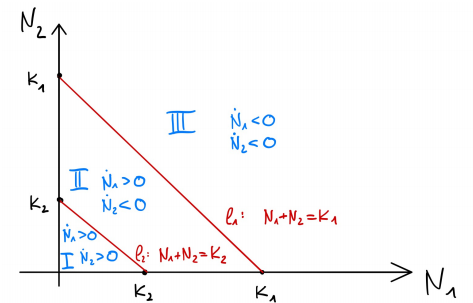
\includegraphics[width=0.3\textwidth]{img/kompetitiver-ausschluss.png}
    \end{center}
    Wenn wir in Gebiet I starten, verlassen wir dieses zu einem späteren Zeitpunkt. 
    Wenn wir in Gebiet II oder III starten, konvergieren wir gegen \((K_1, 0)\).
    Wenn wir in \(l_1\) starten, gehen wir nach II und konvergieren dann. 
\end{karte}